\documentclass{article}
\usepackage[preprint,nonatbib]{neurips_2025}
\usepackage{amsmath,amssymb,booktabs,graphicx,float,hyperref}

\title{DQN and Double DQN for CartPole-v1: A Reproducible DATA8007 Study}
\author{Jianyu Zhang\\Student number: 3030114491}
\date{DATA8007 Foundations of Sequential Decision-Making [2A, 2025]}

\begin{document}
\maketitle

\begin{abstract} This report compares Deep Q-Networks (DQN) and Double DQN on Gymnasium CartPole-v1 using a reproducible PyTorch implementation. Both methods use experience replay, a target network, epsilon-greedy exploration, and identical hyperparameters across three random seeds. The experiments ran on an NVIDIA L40S GPU. Under a 160-episode budget, neither method reached the solved threshold of 475 return. Double DQN achieved higher aggregate returns: its best evaluation return was $250.93 \pm 74.79$, compared with $166.60 \pm 48.91$ for DQN. \end{abstract}
\section{Introduction} Reinforcement learning addresses sequential decision-making problems where an agent learns from rewards produced by interaction with an environment. This project studies value-based deep reinforcement learning on CartPole-v1. DQN is used as the baseline because it extends Q-learning to continuous observations with a neural network. Double DQN is used as the comparison method because it separates action selection from action evaluation in the target, which can reduce overestimation bias.
The research questions are: how reliably DQN improves under fixed hyperparameters, whether Double DQN improves return or evaluation stability, and whether observed differences are robust across seeds. The project is intentionally small so that the full workflow, including training logs, summaries, plots, and report files, can be reproduced from scripts.
\section{Background} A Markov decision process is written as $(\mathcal{S}, \mathcal{A}, P, R, \gamma)$. The discounted return is $G_t=\sum_{k=0}^{\infty}\gamma^k r_{t+k+1}$, and the action-value function is $Q^{\pi}(s,a)=\mathbb{E}_{\pi}[G_t \mid s_t=s,a_t=a]$. The optimal action-value function satisfies $Q^*(s,a)=\mathbb{E}[r+\gamma\max_{a'}Q^*(s',a')]$. DQN approximates this function with a neural network and stabilizes learning with replay and a target network.
\section{Methods} The Q-network is a multilayer perceptron with hidden sizes $[128,128]$ and ReLU activations. The online network is optimized with Adam, learning rate $10^{-3}$, Smooth L1 loss, replay capacity 50,000, batch size 64, discount $\gamma=0.99$, gradient clipping at norm 10, target synchronization every 500 steps, and learning starts after 1,000 steps. Exploration uses epsilon-greedy action selection from 1.0 to 0.05 over 8,000 environment steps.
For DQN, the target is $y^{DQN}=r+\gamma(1-d)\max_{a'}Q_{\theta^-}(s',a')$. For Double DQN, the online network selects $a^*=\arg\max_{a'}Q_{\theta}(s',a')$, while the target network evaluates it as $y^{Double}=r+\gamma(1-d)Q_{\theta^-}(s',a^*)$. This is the only algorithmic difference between the two methods in the experiment.
\section{Experimental Setup} The environment is Gymnasium CartPole-v1, with a four-dimensional continuous observation vector and two discrete actions. Each episode can last up to 500 steps, and the solved threshold is 475 return. Both algorithms use seeds 0, 1, and 2, train for 160 episodes, evaluate every 20 episodes using five greedy episodes, and then evaluate the best checkpoint for 20 episodes with evaluation seed 12345. The run used PyTorch 2.8.0+cu128, Gymnasium 0.29.1, and an NVIDIA L40S GPU. The implementation selects CUDA automatically when available.
\section{Results} The aggregate results in \texttt{results/summary.csv} show that Double DQN outperformed DQN under this budget. DQN obtained final return $90.33 \pm 37.45$, final 50-episode moving average $38.37 \pm 5.46$, and best evaluation return $166.60 \pm 48.91$. Double DQN obtained final return $160.33 \pm 57.84$, final 50-episode moving average $60.09 \pm 17.75$, and best evaluation return $250.93 \pm 74.79$. No run reached the solved threshold.
\begin{table}[H] \centering \caption{Per-seed training summary.} \begin{tabular}{llrrrr} \toprule Method & Seed & Best eval & Final return & Final MA50 & Solved episode \\ \midrule DQN & 0 & 223.0 & 122.0 & 43.56 & -- \\ DQN & 1 & 135.8 & 49.0 & 32.68 & -- \\ DQN & 2 & 141.0 & 100.0 & 38.86 & -- \\ Double DQN & 0 & 295.8 & 205.0 & 76.60 & -- \\ Double DQN & 1 & 292.4 & 181.0 & 41.32 & -- \\ Double DQN & 2 & 164.6 & 95.0 & 62.34 & -- \\ \bottomrule \end{tabular} \end{table}
\begin{figure}[H] \centering 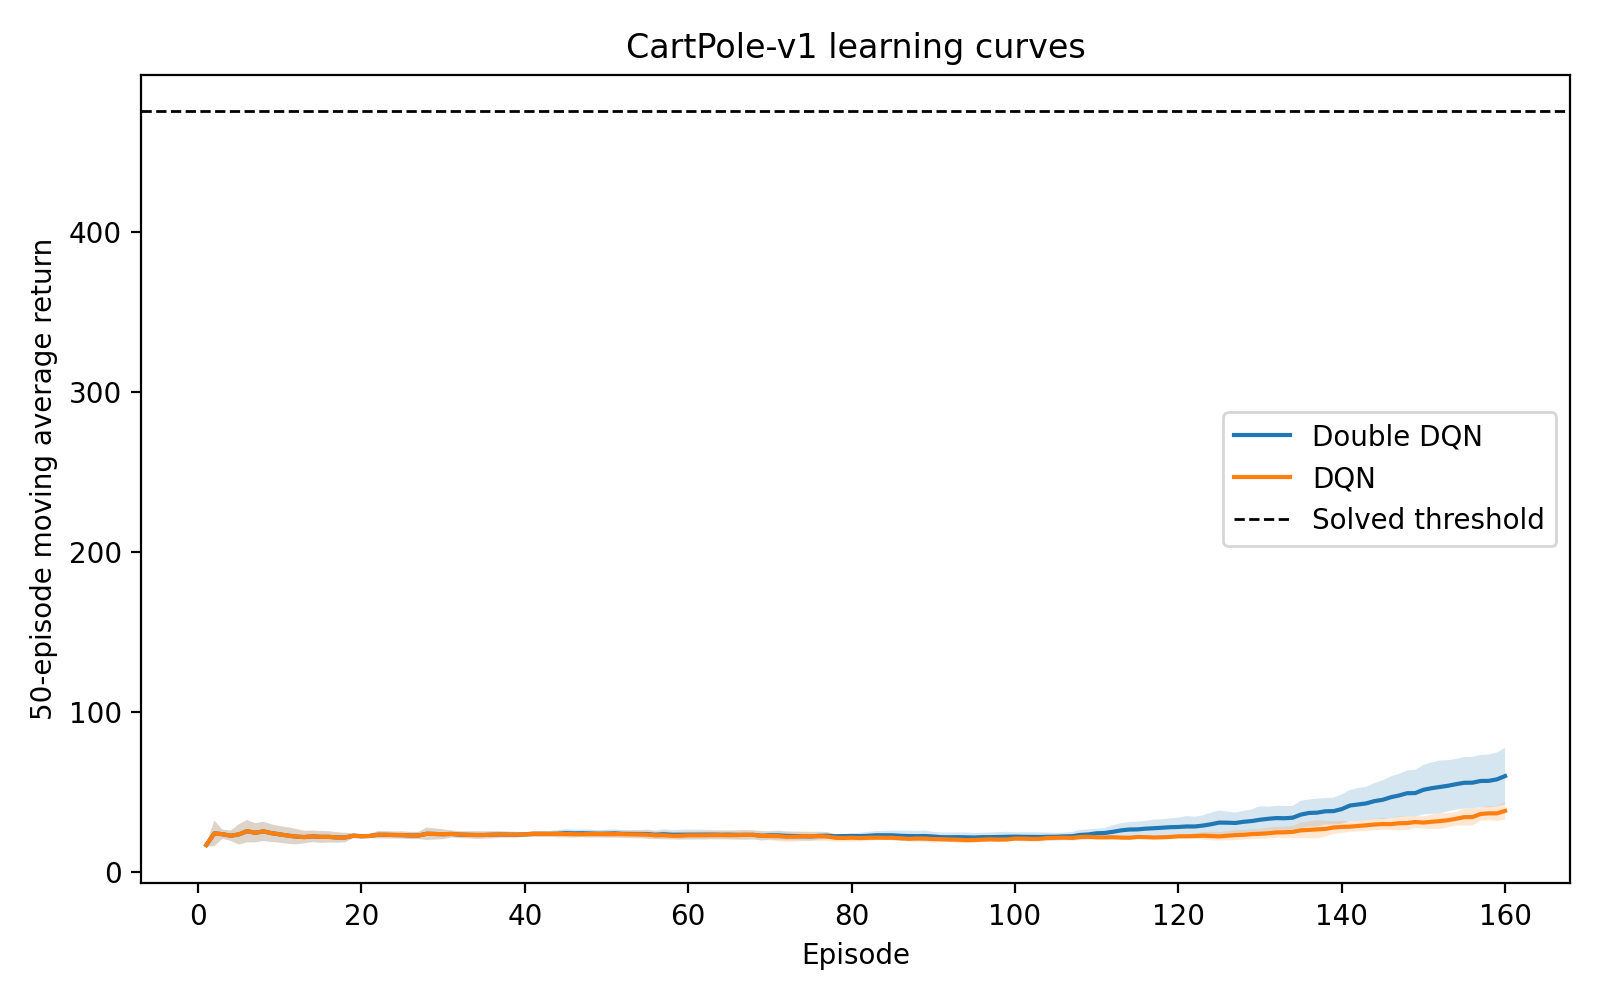
\includegraphics[width=0.85\linewidth]{../results/figures/learning_curves.png} \caption{Training return curves produced from per-seed CSV logs.} \end{figure} \begin{figure}[H] \centering 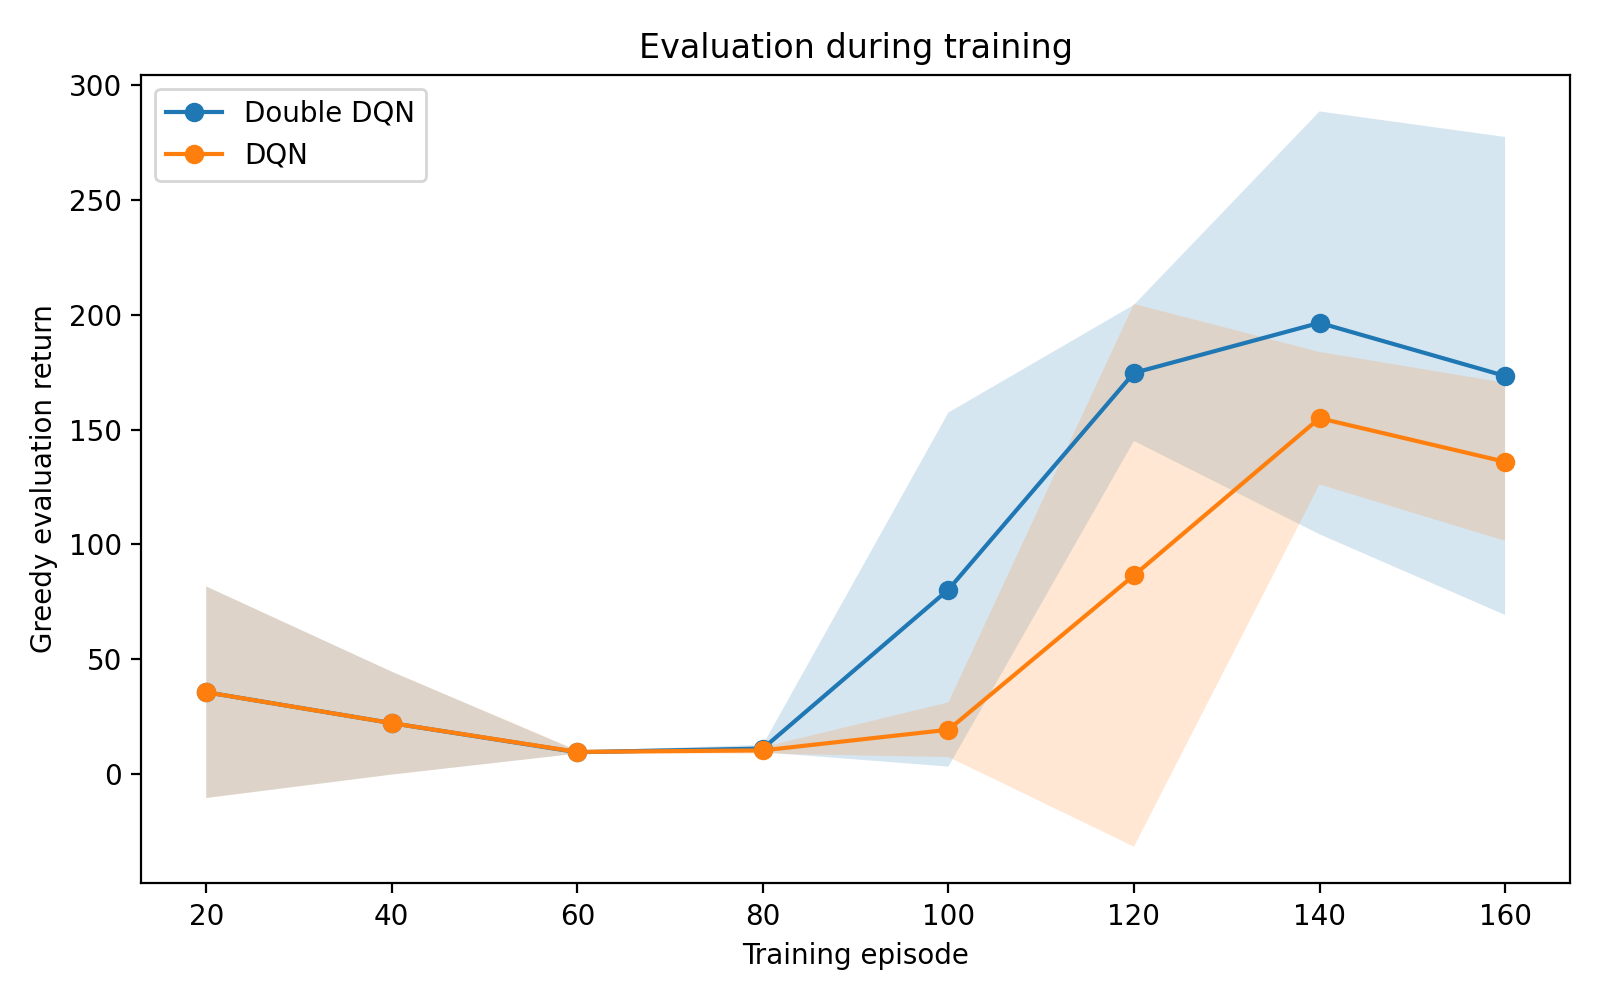
\includegraphics[width=0.85\linewidth]{../results/figures/evaluation_curves.png} \caption{Greedy evaluation returns measured every 20 training episodes.} \end{figure}
The independent 20-episode evaluation of best checkpoints gave DQN seed 0: $176.5 \pm 46.45$, DQN seed 1: $149.2 \pm 11.42$, DQN seed 2: $113.3 \pm 27.99$, Double DQN seed 0: $251.6 \pm 33.90$, Double DQN seed 1: $316.4 \pm 47.40$, and Double DQN seed 2: $152.2 \pm 34.82$. This confirms the same broad pattern while also showing substantial seed sensitivity.
\section{Discussion} The results partially support the expectation that Double DQN can be more stable than DQN. Double DQN has better aggregate performance in this project, especially in best evaluation return. However, the comparison is not decisive because no run solved the environment and the variance across seeds is large. The result should therefore be presented as evidence from a controlled course experiment, not as a general benchmark claim.
The main practical lesson is that even small deep RL experiments can be sensitive to seeds, exploration schedules, replay warmup, and target-network update frequency. A longer training budget, more random seeds, and direct tracking of Q-value overestimation would make the conclusion stronger.
\section{Strengths, Limitations, and Extensions} The project is reproducible: configuration, training, evaluation, plotting, replay buffer, neural network, and agent logic are separated into modules, and all logs, summaries, and figures are saved by scripts. Its limitations are the small benchmark, three-seed sample size, fixed hyperparameters, and short training budget. Natural extensions include more seeds, longer training, prioritized replay, dueling networks, multi-step returns, a policy-gradient baseline, and a harder Gymnasium environment.
\section{Conclusion} This project implements and evaluates DQN and Double DQN for CartPole-v1 in a reproducible PyTorch workflow. Under the selected 160-episode budget, Double DQN produced better aggregate returns than DQN, but no seed reached the solved threshold. The final interpretation is cautious: Double DQN was stronger in this run, while the experiment still shows the seed variance and tuning sensitivity that are common in deep reinforcement learning.
\begin{thebibliography}{9} \bibitem{mnih2015} Volodymyr Mnih et al. Human-level control through deep reinforcement learning. \emph{Nature}, 518:529--533, 2015. \bibitem{hasselt2016} Hado van Hasselt, Arthur Guez, and David Silver. Deep reinforcement learning with Double Q-learning. \emph{Proceedings of the AAAI Conference on Artificial Intelligence}, 2016. \bibitem{gymnasium} Farama Foundation. Gymnasium documentation. \url{https://gymnasium.farama.org/}. \bibitem{pytorch} PyTorch Foundation. PyTorch documentation. \url{https://pytorch.org/}. \end{thebibliography} \end{document}
